\section{Using TrueCrypt}

The following are step-by-step instructions on how to create, mount, and
use a TrueCrypt volume.

\subsection{Creating a TrueCrypt Container}

\begin{enumerate}[1.]
\item
  Install TrueCrypt. Then launch TrueCrypt by

  \begin{itemize}
  \item
    double-clicking the file TrueCrypt.exe in Windows
  \item
    opening
    Applications-\textgreater{}Accessories-\textgreater{}TrueCrypt in
    Ubuntu
  \item
    on MacOSX open it by clicking Go \textgreater{} Applications. Find
    TrueCrypt in the Applications folder and double click on it.
  \end{itemize}
\item
  When the main TrueCrypt window appears. Click Create Volume.
\end{enumerate}
\begin{figure}[htbp]
\centering
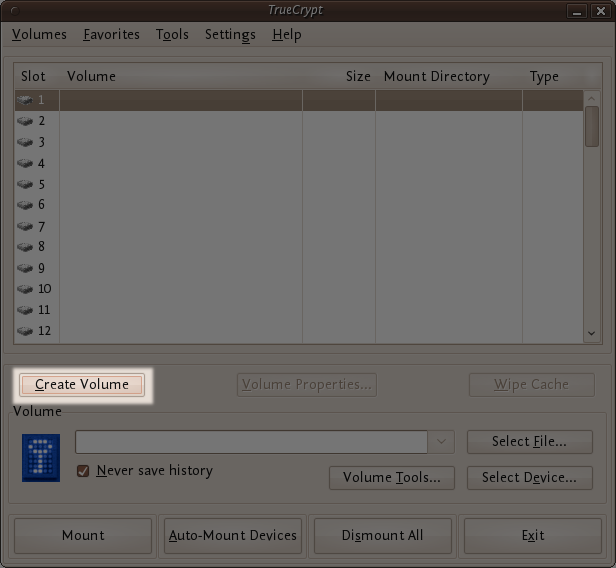
\includegraphics{using_tc_001.png}
\caption{Using TrueCrypt}
\end{figure}

\begin{enumerate}[1.]
\setcounter{enumi}{2}
\item
  You should see the TrueCrypt Volume Creation Wizard window appear on
  screen.
\end{enumerate}
\begin{figure}[htbp]
\centering
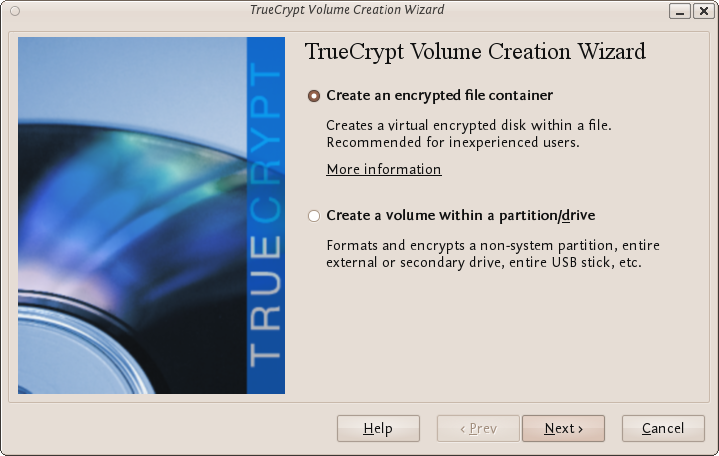
\includegraphics{using_tc_002.png}
\caption{Using TrueCrypt}
\end{figure}

Where do you want to create the TrueCrypt volume? You need to choose
now. This can be in a file, which is also called a container, in a
partition or drive. The following steps will take you through the first
option creating a TrueCrypt volume within a file.

You can just click Next, as the option is selected by default,

\begin{enumerate}[1.]
\setcounter{enumi}{3}
\item
  Next you need to choose whether to create a standard or hidden
  TrueCrypt volume. We will walk you through the former option and
  create a standard TrueCrypt volume.
\end{enumerate}
\begin{figure}[htbp]
\centering
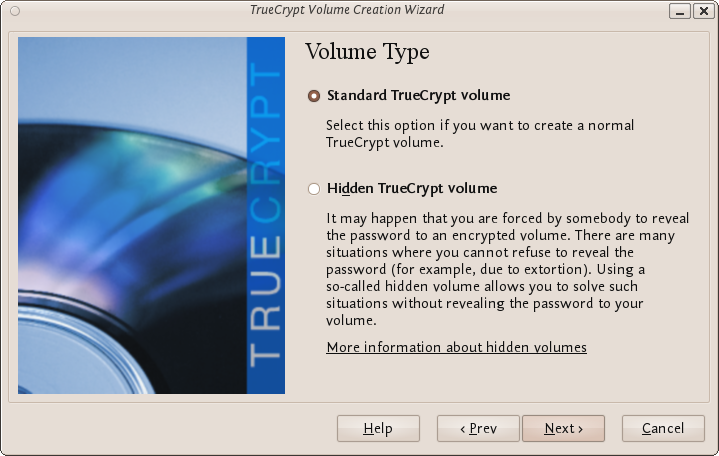
\includegraphics{using_tc_003.png}
\caption{Using TrueCrypt}
\end{figure}

You can just click Next, as the option is selected by default.

\begin{enumerate}[1.]
\setcounter{enumi}{4}
\item
  Now you have to specify where to have the TrueCrypt volume (file
  container) created. Note that a TrueCrypt container behaves like any
  normal file. It can be moved or deleted as any normal file.
\end{enumerate}
\begin{figure}[htbp]
\centering
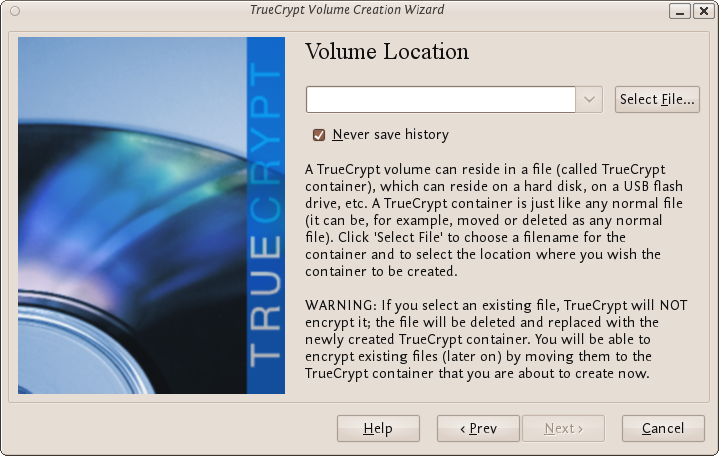
\includegraphics{using_tc_004.png}
\caption{Using TrueCrypt}
\end{figure}

Click Select File.

The standard file selector will now appear on screen (the TrueCrypt
Volume Creation Wizard remains open in the background). You need to
browse to the folder that the file should be created in and then type
into the `name' field the name for the file you wish to create.

\begin{figure}[htbp]
\centering
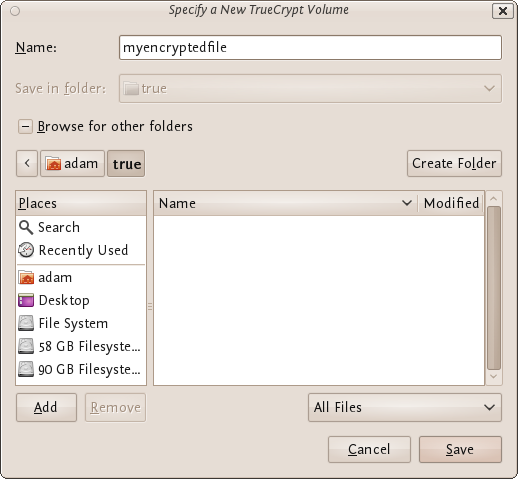
\includegraphics{using_tc_005.png}
\caption{Using TrueCrypt}
\end{figure}

We will create our TrueCrypt volume in the folder `adam/true' and the
filename of the volume (container) will be `myencryptedfile'. You may,
of course, choose any other filename and location you like (for example,
on a USB stick). Note that the file `myencryptedfile' does not exist yet
- TrueCrypt will create it. Press `Save' when you are ready. The file
selector window should close.

\textbf{IMPORTANT:} Note that TrueCrypt will not encrypt any existing
files. If an existing file is selected in this step, it will be
overwritten and replaced by the newly created volume (the contents of
the existing file will be lost). You will be able to encrypt existing
files later on by moving them to the TrueCrypt volume that we are
creating now.

\begin{enumerate}[1.]
\setcounter{enumi}{5}
\item
  In the Volume Creation Wizard window (which was previously running in
  the background), click Next.
\item
  Here you can choose an encryption algorithm and a hash algorithm for
  the volume.
\end{enumerate}
\begin{figure}[htbp]
\centering
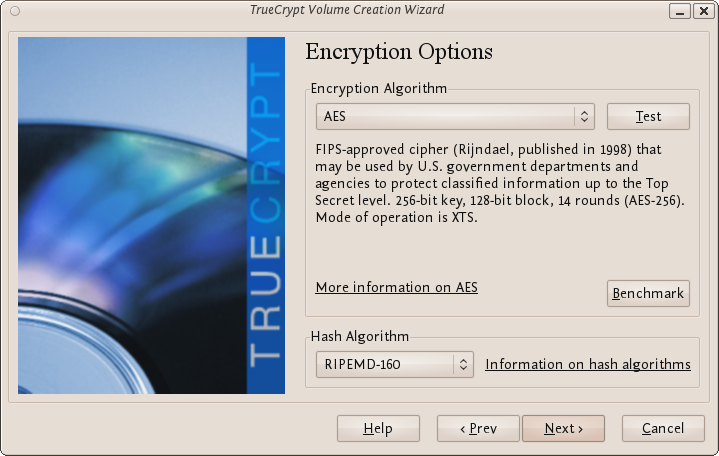
\includegraphics{using_tc_006.png}
\caption{Using TrueCrypt}
\end{figure}

The TrueCrypt manual suggests that if you are not sure what to select
here, you can use the default settings and click Next (for more
information about each setting have a look at the TrueCrypt
documentation website).

\begin{enumerate}[1.]
\setcounter{enumi}{7}
\item
  Now choose the size of your container. You should be fine with 1
  megabyte but for this example we will enter `20' into the available
  field.
\end{enumerate}
\begin{figure}[htbp]
\centering
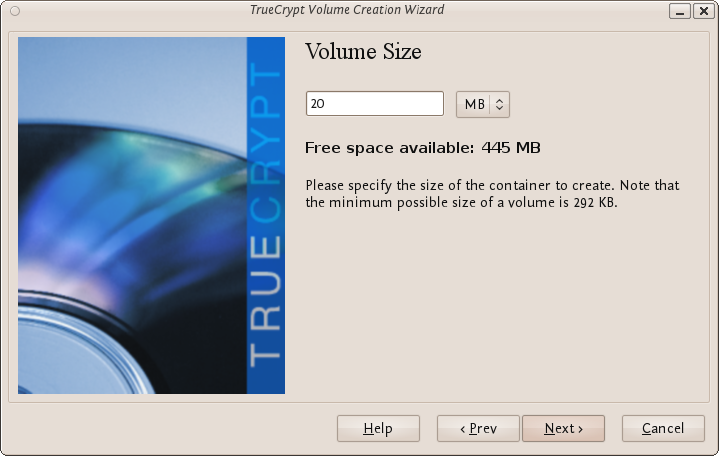
\includegraphics{using_tc_007.png}
\caption{Using TrueCrypt}
\end{figure}

You may, of course, specify a different size. After you type the desired
size in the input field, click Next.

\begin{enumerate}[1.]
\setcounter{enumi}{8}
\item
  This step is really important, choosing a password.
\end{enumerate}
The information displayed in the Wizard window about what is considered
a good password, should be read carefully.

Choose a strong password, type it in the first input field. Then re-type
it in the input field below the first one.

\begin{figure}[htbp]
\centering
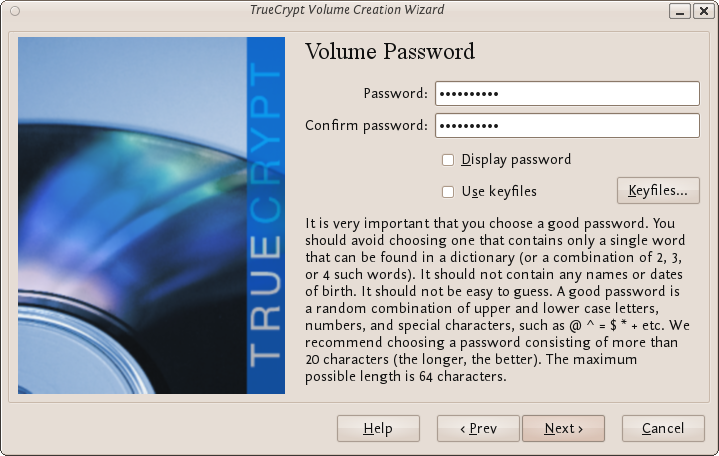
\includegraphics{using_tc_008.png}
\caption{Using TrueCrypt}
\end{figure}

When you are done click Next.

\begin{enumerate}[1.]
\setcounter{enumi}{9}
\item
  Now you must choose the format of your partition (this step may not be
  available for you under windows or OSX). If using Ubuntu you can
  choose a Linux file type or FAT (Windows) for simplicity leave it at
  the default.
\end{enumerate}
\begin{figure}[htbp]
\centering
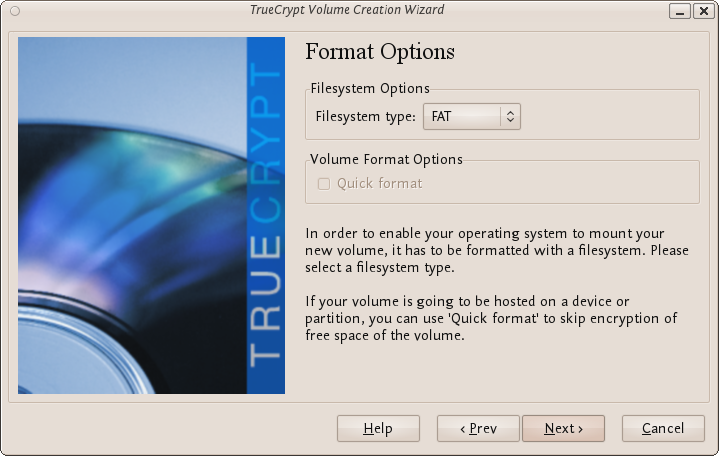
\includegraphics{using_tc_009.png}
\caption{Using TrueCrypt}
\end{figure}

Then press Next.

\begin{enumerate}[1.]
\setcounter{enumi}{10}
\item
  Next TrueCrypt tries to generate random information to help encrypt
  your container. For 30 seconds move your mouse as randomly as possible
  within the Volume Creation Wizard window. Move the mouse as much as
  possible for up to a minute. This significantly increases security by
  increasing the cryptographic strength of the encryption keys.
  security). Move your mouse around until you are bored.
\end{enumerate}
\begin{figure}[htbp]
\centering
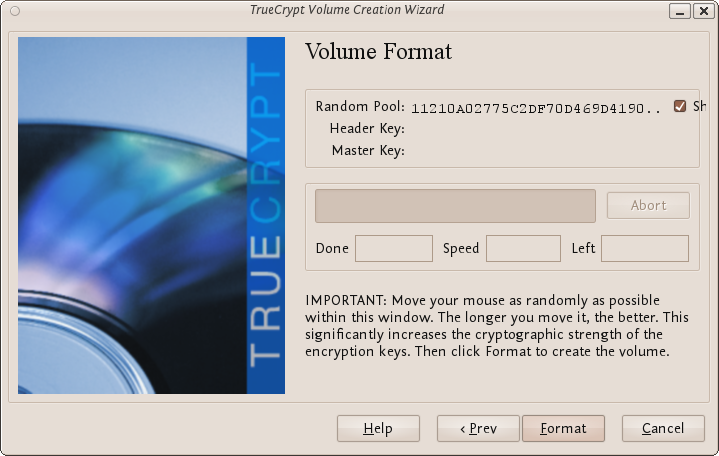
\includegraphics{using_tc_010.png}
\caption{Using TrueCrypt}
\end{figure}

Then Click Format.

TrueCrypt will now create a file in the folder you selected with the
name you chose. This file will be a TrueCrypt container, containing the
encrypted TrueCrypt volume. This may take some time depending on the
size of the volume. When it finishes this should appear:

\begin{figure}[htbp]
\centering
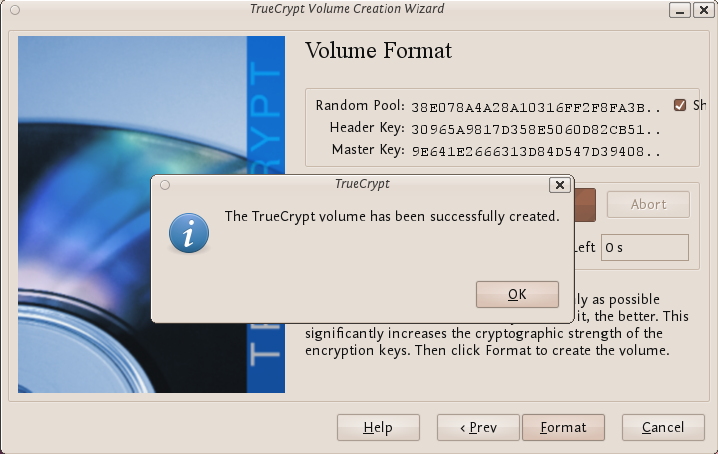
\includegraphics{using_tc_011.png}
\caption{Using TrueCrypt}
\end{figure}

Click OK to close the dialog box.

\begin{enumerate}[1.]
\setcounter{enumi}{11}
\item
  Well done! You've just successfully created a TrueCrypt volume (file
  container).
\end{enumerate}
In the TrueCrypt Volume Creation Wizard window, click Exit.

\subsection{Mounting the Encrypted Volume}

\begin{enumerate}[1.]
\item
  Open up TrueCrypt again.
\item
  Make sure one of the `Slots' is chosen (it doesn't matter which - you
  can leave at the default first item in the list). Click Select File.
\end{enumerate}
\begin{figure}[htbp]
\centering
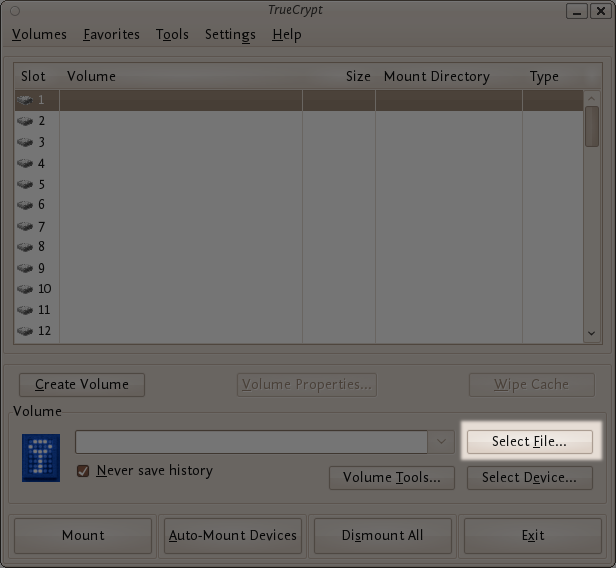
\includegraphics{using_tc_012.png}
\caption{Using TrueCrypt}
\end{figure}

The standard file selector window should appear.

\begin{enumerate}[1.]
\setcounter{enumi}{2}
\item
  In the file selector, browse to the container file (which we created
  earlier) and select it.
\end{enumerate}
\begin{figure}[htbp]
\centering
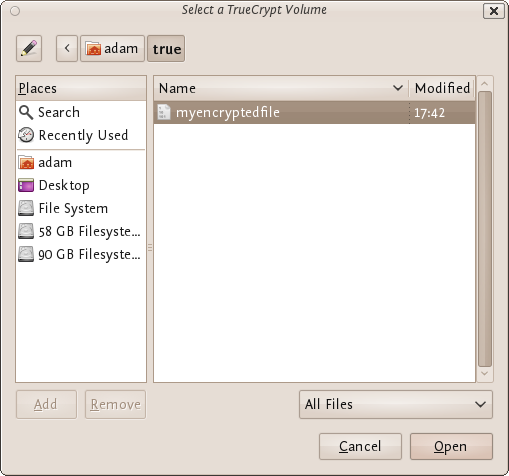
\includegraphics{using_tc_013.png}
\caption{Using TrueCrypt}
\end{figure}

Click Open (in the file selector window).

The file selector window should disappear.

\begin{enumerate}[1.]
\setcounter{enumi}{3}
\item
  In the main TrueCrypt window, click Mount.
\end{enumerate}
\begin{figure}[htbp]
\centering
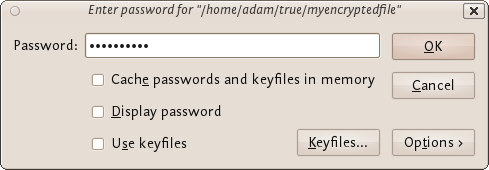
\includegraphics{using_tc_014.png}
\caption{Using TrueCrypt}
\end{figure}

Password prompt dialog window should appear.

\begin{enumerate}[1.]
\setcounter{enumi}{4}
\item
  Type the password in the password input field.
\end{enumerate}
\begin{figure}[htbp]
\centering
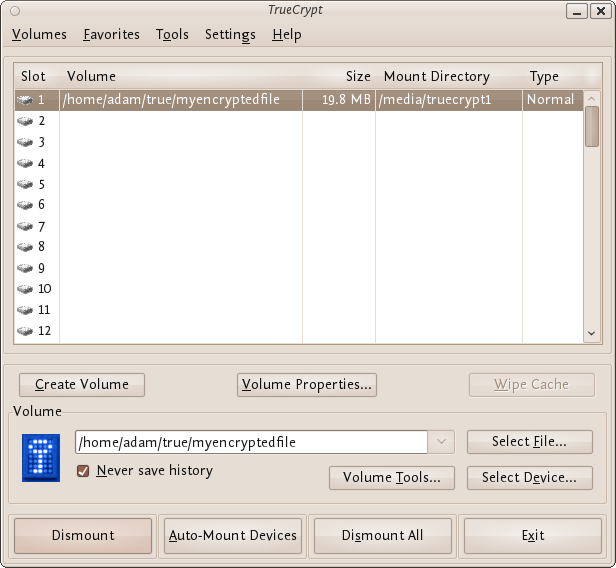
\includegraphics{using_tc_015.png}
\caption{Using TrueCrypt}
\end{figure}

\begin{enumerate}[1.]
\setcounter{enumi}{5}
\item
  Click OK in the password prompt window.
\end{enumerate}
TrueCrypt will now attempt to mount the volume. If the password is
correct, the volume will be mounted.

\begin{figure}[htbp]
\centering
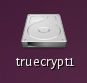
\includegraphics{using_tc_016.png}
\caption{Using TrueCrypt}
\end{figure}

If the password is incorrect (for example, if you typed it incorrectly),
TrueCrypt will notify you and you will need to repeat the previous step
(type the password again and click OK).

\begin{enumerate}[1.]
\setcounter{enumi}{6}
\item
  We have just successfully mounted the container as a virtual disk 1.
  The container will appear on your Desktop or you will see it in your
  file browser.
\end{enumerate}
\subsection{What does this mean?}

The disk that you have just created is completely encrypted and behaves
like a real disk. Saving (moving, copying, etc) files to this disk will
allow you to encrypt files on the fly.

You'll be able to open a file which is stored on a TrueCrypt volume,
which will automatically be decrypted to RAM while it is being read, and
you won't need to enter your password each time. You'll only need to
enter this when your mounting the volume.

\subsection{Remember to dismount!}

To do this right click on the drive and select unmount. This will
automatically happen when you turn off your computer but will not happen
if you just put the computer on sleep.
